\begin{document}
\chapter{Aplicatia MyMusicTeacher}

\section{Definirea problemei}
	Problema tratata de aceasta lucrare de licenta o reprezinta detectarea vizuala a notelor muzicale pe partitura, in timp real, folosind camera unui dispozitiv mobil. 
	
	Propunem crearea unui sistem inteligent, ce poate fi transpus si poate functiona la parametri optimi pe o gama cat mai larga de dispozitive mobile. Acest sistem va primi, in mod continuu, date de intrare de la camera video a dispozivului mobil, va procesa in timp real imaginile, si va aduce o predictie pentru fiecare cadru, reprezentand nota muzicala prezenta pe partitura. 
	
	Dorim sa excludem dependenta conexiunii la internet la momentul procesarii imaginilor, iar in acest scop propunem creearea unui modul, compatibil cu dispozitive mobile, care sa lucreze izolat cu parametrii optimizati de catre sistemul inteligent, creat si antrenat pe server, si un serviciu care ruleaza pe o masina cu acces la internet, capabila de a transmite aplicatiilor de pe dispozitivile mobile, parametrii sistemului inteligent. 
	
	Dorim ca sistemul inteligent, prezent pe telefon, sa poata fi actualizat cu usurinta prin intermediul serviciului.  

\section{Analiza problemei}
	In scopul rezolvarii acestei probleme, vom urmari si defini un numar de pasi, pentru a modela aplicatia si functionalitatile sale.
	Pentru primul pas in scopul rezolvarii acestei probleme, ne vom folosi de ramura invatarii automate, specializata in procesarea de imagine. Vom profita de eficienta, la nivel de timp si memorie, al retelelor neuronale convolutionale si vom implementa o aplicatie, care permite configurarea si antrenarea unui model.
	
	Aplicatia va rula pe un sistem cu capacitate computationala buna. Aceasta va permite construirea arhitecturii modelului de retele neuronale convolutionale si  alegerea unor parametrii utilizati pe parcursul procesului de invatare, iar pe baza configuratiei alese  va trece modelul prin etapa de antrenare. La finalul  etapei de antrenare, aplicatia va crea un fisier de tip JSON, unde va exporta arhitectura modelului impreuna cu parametrii acestuia. 
	
	Exportarea fisierului JSON, unde este prezenta o versiune a modelului antrenat, este realizata in scopul plasarii acestui model pe un server, responsabil cu departajarea informatiilor tuturor clientilor. 
	Pentru antrenarea modelului, vom folosi un set de aproximativ 800 de poze, realizate cu un dispozitiv mobil si pre-procesate in scopul scoaterii in evidenta a informatiei relevante. Pozele vor fi grupate in  7 clase, reprezentand note intregi, simple (fara diez si bemol), de la DO la SI, avand cca. 120 de poze per clasa. 
	
	Aplicatia va incarca in memorie imaginile, le va procesa pentru a le aduce la dimensiunea optima antrenarii si va gestiona dimensiunile canalelor de imagine, in scopul optimizarii complexitatii de timp al etapei de invatare. Dupa realizarea acestor pasi, aplicatia va trece setul de date de intrare printr-o etapa de randomizare, cu scopul inlaturarii omogenitatii, un factor crucial care influenteza capabilitatea modelului de atingere a unei precizii optime, iar pe baza configuratiei alese aplicatia va grupa imaginile si le va transmite modelului in scopul antrenarii.
	
	Aplicatia va permite monitorizarea, in timp real, a progresului modelului si a preciziei acumulate. La finalul etapei de antrenare, vom exporta intr-un fisier progresul antrenarii, asemanator unui istoric, in eventuala posibilitate de a analiza progresul fiecarui model dupa etapa de antrenare.
	Scopul aplicatiei va fi: modelarea unei arhitecturi cu o precizie cat mai ridicata.
	Configurarile valabile vor fi:
	
	\begin{itemize}
	\item	Alegerea dimensiunii seturilor de antrenare (batch size). Acest parametru va gestiona modul de grupa a grupurilor de imagini. In functie de acest parametru se vor calcula numarul de iteratii si dimensiunea setului de date de validare.
	
	
	\item	Construirea arhitecturii prin adaugarea si configurarea straturilor retelei neuronale convolutionale (layers).  Fiecare strat al retelei, va fi configurat individual si va fi adaugat in arhitectura modelului. Tipurile de straturi care vor fi prezente in aplicatie sunt: Convolution Layer, Max Pooling Layer, Flattening Layer si Hidden Layer. Aceste straturi vor fi configurate prin parametrii cum ar fi: dimensiunea ponderilor, dimensiunea si numarul filtrelor, step-size (forta de modificare a ponderilor si a filtrelor), parametru de regularizare, etc.
	
	\item	Alegerea unui clasificator capabil de creearea unei predictii, bazate pe datele procesate anterior de catre straturile modelului. Desi  natura aplicatiei permite alegerea mai multor tipuri de clasificatoare in etapa de construire a arhitecturii, vom implementa clasificatorul Softmax, avand o eficienta ridicata in cazul contextului nostru.
	
	\item	Configurarea parametrilor specifici etapei de antrenare: numarul de iteratii, numarul de imagini ce vor fi date spre procesare, etc.
	
	\end{itemize}

	Al doilea pas, in scopul rezolvarii problemei propuse, este de a crea un serviciu backend, care va fi capabil de a gestiona si transmite modelul creat. O metoda eficienta de a realiza acest lucru, ar fi implementarea unui serviciu de tip REST api, care este capabil de a transmite fisierul creat de model, in format JSON, direct prin expunerea sa ca resursa. 
	Un avantaj considerabil al utilizarii un serviciu backend, este posibilitatea de actualizare a modelului, printr-o simpla schimbare a resursei prezente pe server cu una noua, creata de aplicatia noastra responsabila cu antrenarea modelului. 
	
	Al treilea pas, in scopul rezolvarii problemei propuse, este crearea unui modul compatibil cu dispozitivele mobile, responsabil de integrarea modelului transmis si utilizarea sa in scopul obtinerii unei predictii. 
	Acest modul se va ocupa strict cu partea de inferenta a modelului si nu va fi dependent de modul in care sunt gestionate imaginile de la camera dispozitivului mobil sau de modul in care este adus  modelul pe dispozivitul mobil. Implementarea sa va fi echivalentul implementarii aplicatiei de construire si antrenare al sistemului inteligent, dar va fi exclusa partea de construire a arhitecturii si de antrenare. 
	Propunem integrarea modulului de inferenta, printr-o componenta independenta de aplicatie. In acest mod, separam functionalitatile de baza ale aplicatiei si permitem reutilizarea sau chiar schimbarea componentei de inferenta intr-un mod mult mai accesibil.
	
	Al patrulea pas in rezolvarea problemei propuse, este crearea unei aplicatii mobile, care va utiliza modulul de inferenta si modelul transmis de server, in scopul crearii unor predictii bazate pe imagini aprovizionate in mod repetitiv, prin intermediul camerei dispozitivului.  
	Aplicatia va fi dezvoltata pe sistemul de operare Android, si va folosi interefete native pentru gestionarea si procesarea imaginilor de la camera. 
	Propunem o interfata vizuala minimala si sugestiva, care va coordona utilizatorul in utilizarea functionalitatilor propuse. Utilizatorul poate alege cand sa fie procesate imaginile, prin apasarea unui buton de tip toggle. 
	Aplicatia isi va aproviziona sau isi va actualiza modelul prin intermediul serviciului, odata cu fiecare pornire, daca dispozitivul este conectat la internet. 

	\section{Proiectare}
	
	Aplicatia este constituita dintr-un numar de 4 componente, concepute pentru a lucra impreuna: 
	
	\begin{itemize}	
	\item	Aplicatia Python responsabila cu  antrenarea modelului de retele neuronale
	\item	Modulul de inferenta scris in Java pentru portarea modelului de dispozitive mobile
	\item	Serviciu Java REST API, pentru distribuirea modelului
	\item	Aplicatie client Android care utilizeaza modelul pentru recunoasterea notelor muzicale
	\end{itemize}
	
	\subsection{Antrenarea modelului}
	
	Pentru implementarea aplicatiei de antrenare al modelului am utilizat limbajul de programare Python, un limbaj consacrat domeniului inteligentei artificiale, biblioteca Pillow, continand implementarea unor functionalitati responsabile de procesarea imaginilor, de care am avut nevoie in etapa de incarcare in memorie si pre-procesare a imaginilor si biblioteca NumPy care contine implementari eficiente, a operatiilor matematice de care am avut nevoie pe parcursul pasului de antrenare si inferenta. 
	
	\vfill
	
	Scopul principal al aplicatiei este de a expune o interfata de programare, capabila de a defini structura si arhitectura unei retele neuronale, cu posibilitatea extinderii spre functionalitatea de convolutie. Pentru a realiza acest lucru, aplicatia noastra defineste 4 entitati de baza, care implementeaza modul de functionare al straturilor unei retele neuronale. 
	
	Implementarea a fost facuta respectand principiile programarii orientate obiect, in scopul mentinerii unei structuri human-friendly a codului si definirea concreta a entitatilor. Astfel fiecare strat va fi reprezentat de o clasa: HiddenLayer, ConvLayer si PoolingLayer. 
	
	Deoarece logica de manipulare a datelor de intrare si logica de mutatie a ponderilor difera de la un tip de strat la celalalt, am utilizat proprietati ale polimorfismului pentru a putea usura etapa de antrenare a modelului. Astfel fiecare entitate va implementa in structura sa metodele abstracte necesare pentru circulatia datelor. 
	
	Conceptul feed-forward este ceea ce ne permite sa cream o mutatie asupra datelor de intrare, utilizand ponderi. 
	Operatia de tip forward, realizata de un strat de tip Hidden va fi realizata astfel: 
	
	\begin{itemize}
	\item	Se considera datele de intrare ca fiind o matrice bi-dimensionala. Fiecare linie va corespunde unei intrari, i.e un vector de valori.
	
	\item	Stratul Hidden defineste o matrice bi-dimensionala, reprezentand ponderile fiecarui neuron, pe coloane. Operatia de inmultire a matricilor (utilizand metoda dot a bibliotecii NumPy) avand ca operanzi datele de intrare (matrice de bidimensionala, avand cate o intrare pe fiecare linie) si ponderile (matrice bidimensionala, avand ponderile fiecarui neuron pe coloana) se va demonstra a fi echivalentul operatiilor pe care neuronii artificiali le realizeaza.  Inmultind liniile primei matrici cu coloanele celei de a doua matrici si insumandule, obtinem exact rezultatul pe care un neuron il obtine insumand datele de intrare ponderate. 
	
	
	\item	Rezultatul obtinut va contine pe fiecare linie datele de iesire procesate de neuroni. Acest rezultat va fi trecut printr-o functie de activare, in scopul perturbarii linearitatii operatiei de insumare. Despre modul de functionare al functiei si tipurilor de activare vom discuta mai tarziu in lucrare.
	
	\item	Dupa realizarea acestor pasi, suntem pregatiti sa trimitem rezultatul mai departe spre a fi procesat de eventuale urmatoare straturi. (Vezi Fig. \ref{fig:hidden_forward}).
	\end{itemize}

	
	\begin{figure}[H]
		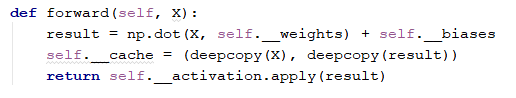
\includegraphics[width=14cm]{hidden_forward}  
		\caption{\label{fig:hidden_forward} Operatia forward a clasei HiddenLayer}
	\end{figure}

	\newpage
	
	Stratul de tip Convolution va avea o perspectiva diferita asupra functiei follow:
	\begin{itemize}
		
	\item	 De data aceasta datele de intrare vin de forma unei matrici 4-dimensionale. Prima dimensiune este responsabila pentru stocarea datelor de intrare, reprezentate de data aceasta sub forma unei matrici 3-dimensioanle (o matrice cu multiple canale de valori ale pixelilor sau un feature-map).
	
	\item	Clasa va detine si va defini o matrice 3-dimensionala, reprezentand filtrele de convolutie. Asemanator datelor de intrare, fiecare element din prima dimensiune a matricii este un filtru de forma unei matrici bi-dimensionale. In scopul usurarii procesarii operatiilor de convolutie, despre care vom discuta in cele ce urmeaza, filtrele vor fi de forma 1X(n*n), unde n este dimensiunea filtrului.
	
	
	\item	Pentru a realiza operatia de convolutie am recurs la abordarea folosind functiile im2col, respectiv col2im. Scopul operatiei im2col, este de a rearanja structura matricii de intrare, astfel incat operatia de convolutie sa fie redusa la o inmultire de matrici.
	
	\item	Odata ce datele de intrare au fost procesate si remodelate de catre functia im2col, vom realiza o inmultire de matrici cu datele remodelate si filtrele stratului. Dupa aplicarea operatiei de col2im pentru restabilirea formei initiale, vom obtine rezultatul convolutiei filtrelor asurpa datelor de intrare.
	
	
	\item	Dorim ca operatia de convolutie sa nu reduca dimensiunea datelor de intrare. Pentru respectarea acestei constrangeri, atributului zeroPadding, al clasei ConvLayer, ii va fi setat, odata cu initializarea obiectului, o valoare care reprezinta numarul de coloane si randuri de 0 ce trebuiesc adaugate datelor de intrare pentru a-si pastra forma dupa operatia de convolutie.
	
	\item	Dupa finalizarea operatiei de convolutie, vom readuce rezultatul in forma initiala utilizand functia col2im, vom aplica functia de activare si vom returna valoarea. 	(Vezi Fig. \ref{fig:conv_forward})

	\end{itemize}

	\vfill
	
	\begin{figure}[H]
		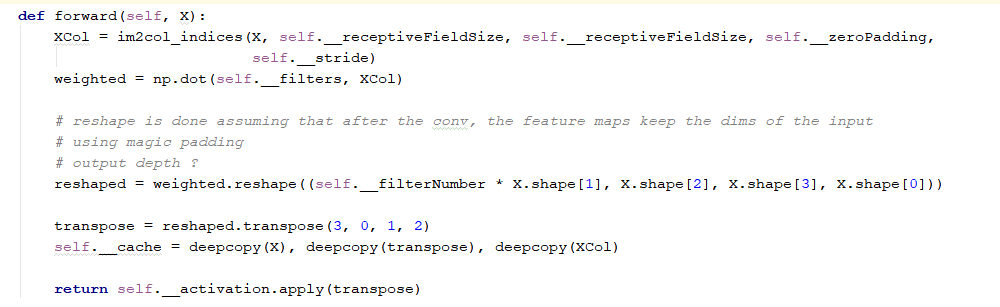
\includegraphics[width=14cm]{conv_forward}  
		\caption{\label{fig:conv_forward} Operatia forward a clasei ConvLayer}
	\end{figure}

	
	Stratul de tip Pooling, desi asemanator stratului de tip Convolution, defineste follow astfel:
	
	\begin{itemize}
	\item	Datele de intrare vor avea aceeasi forma ca si la stratul de tip Convolution. 
	
	\item	Vom reutiliza functia im2col datorita operatiei de Max Pooling, care este o operatie asemanatoare convolutiei. Aplicand functia argmax, a bibliotecii NumPy, pe rezultatul functiei im2col, vom obtine pozitia fiecarui element cu valoare maxima de pe fiecare coloana, i.e rezultatul maxim in interiorul fiecarui portiuni posibile operatiei de convolutie. 
	
	\item	Odata ce avem pozitiile fiecarui element maxim, vom crea, pentru fiecare data de intrare, o matrice noua care contine doar elementele cu valoarea maxima. Rezultatul obtinut reprezinta o versiune cu o dimensiune redusa fata de cea initiala si cu detalii mai pronuntate. La finalul procesarii returnam rezultatul.	(Vezi Fig. \ref{fig:pool_forward})
	\end{itemize}

	\vfill
	
	\begin{figure}[H]
		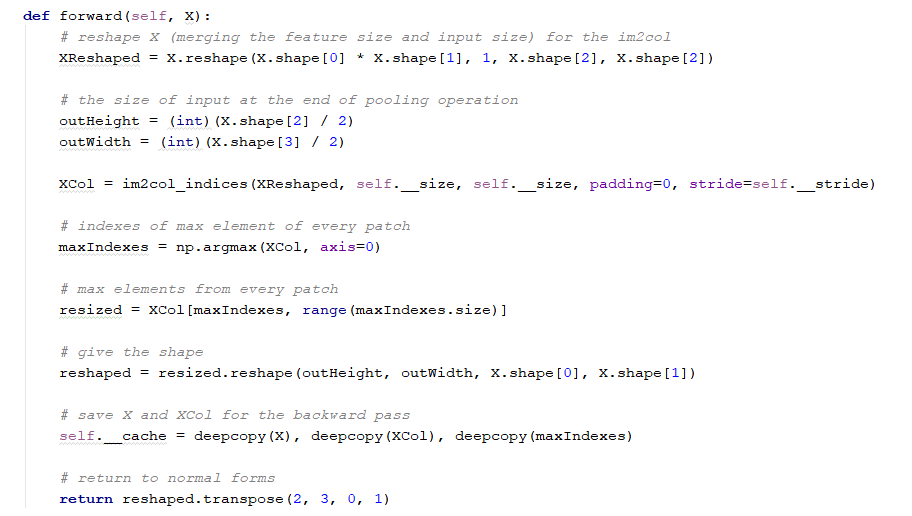
\includegraphics[width=15cm, height=7cm]{pool_forward}  
		\caption{\label{fig:pool_forward} Operatia forward a clasei PoolingLayer}
	\end{figure}
	
	
	In scopul rezolvarii incompatibilitatii intre cele doua tipuri de straturi, Convolution si Hidden, la nivelul datelor de intrare si iesire, introducem un tip de strat a carui functie forward, este responsabil de conversia intre cele doua reprezentari.
	 
	Pentru a realiza conversia, am folosit metoda reshape a componentelor de tip numpy.ndarray. (Vezi Fig. \ref{fig:reshape})
	
	\begin{figure}[H]
		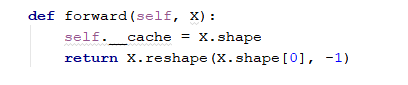
\includegraphics[width=10cm]{reshape}  
		\caption{\label{fig:reshape} Operatia forward a clasei FlatteningLayer}
	\end{figure}
	
	In momentul in care datele de intrare au finalizat un circuit prin lantul de straturi configurat, iar mutatiile au fost aplicate, este momentul sa folosim un clasificator pentru a obtine o decizie. 
	
	Aplicatia defineste un singur tip de clasificator, in scopul contextului problemei noastre, dar permite adaugarea sau implementarea mai multor tipuri de clasificatoare pe aceeasi idee a conceptului de polimorfism. 
	
	Ultimului strat adaugat in configuratie, ii revine datoria de a reduce dimensiunea de iesire dupa procesare, la numarul de clase ce trebuiesc clasificate. Acest lucru in cazul nostru este realizat de un strat de tip Hidden care are n ca dimensiune de iesire si k dimensiune de iesire (unde n este dimensiunea datelor de iesire al stratului precedent iar k este numarul total de clase ce trebuiesc clasificate).
	 
	Implementarea functiei Softmax de clasficiare se face in clasa Softmax din pachetul model. Algoritmul foloseste functia exponent al bibliotecii NumPy pentru a reprezenta valorile obtinute sub forma de probabilitati, iar mai apoi le normalizeaza. (Vezi Fig. \ref{fig:softmax})
	
	\vfill
	
	\begin{figure}[H]
		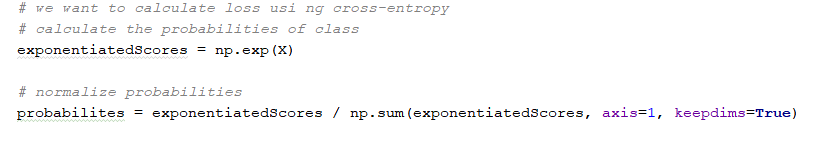
\includegraphics[width=10cm]{softmax}
		\caption{\label{fig:softmax} Cod sursa pentru algoritmul Softmax}
	\end{figure}

	\newpage
	
	Dupa finalizarea acestor pasi, vom obtine pentru fiecare intrare un vector de dimensiune k care contine probabilitatea pentru fiecare clasa pe pozitia i ( 0 >= i > k, unde k este numarul de clase). Datorita faptului ca avem doar o singura clasa corecta, corespunzatoare fiecarei data de intrare, cunoscuta in momentul antrenarii, dorim sa aflam cum a influentat modelul nostru decizia si cum putem sa il penalizam, in cazul unei decizii eronate. Pentru a realiza acest lucru, vom calcula functia de eroare cross-entropy (Vezi Fig. \ref{fig:cross-entropy}). Avantajul utilizarii acestei functii de eroare, este valoarea sa descrecatoare exponential, pe masura ce x creste. (Vezi Fig. \ref{fig:logloss})
	
	\begin{figure}[H]
		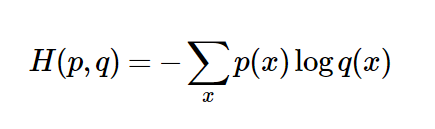
\includegraphics[width=10cm]{cross-entropy}
		\caption{\label{fig:cross-entropy} Functia cross-entropy, unde p este un vector cu clasele corecte iar q este un vector cu predictiile modelului}
	\end{figure}	
	
	\vfill
	
	\begin{figure}[H]
		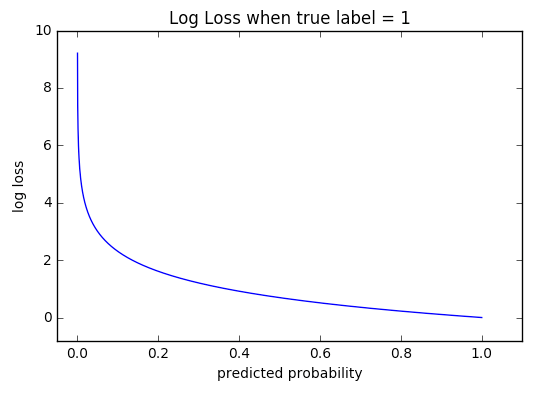
\includegraphics[width=10cm]{logloss}
		\caption{\label{fig:logloss} Reprezentare grafica a functiei de eroare logaritm}
	\end{figure}


	Scopul final al utilizarii acestei functii de eroare, este de a obtine valorile de penalizare ce trebuiesc aplicate ponderilor ce au influentat aceasta decizie. (vezi Fig. \ref{fig:error})
	
	\begin{figure}[H]
		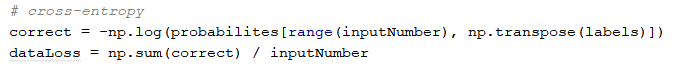
\includegraphics[width=14cm]{error}
		\caption{\label{fig:error} Calcularea erorii prin functia logaritm}
	\end{figure}

	
	Implicit, clasificatorul Softmax va calcula functia de regularizare L2, utilizand parametrul configurat regularization, asupra ponderilor straturilor configurate. Functia L2 ne va da o valoare reprezentand eroarea de regularizare, care va urma a fi adaugata la eroarea functiei logaritm in scopul evitarii situatiei de overfitting. (vezi Fig. \ref{l2})


	\begin{figure}[H]
		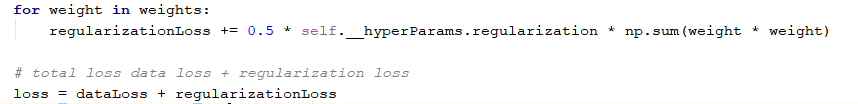
\includegraphics[width=15cm]{l2}
		\caption{\label{fig:l2} Calcularea regularizarii L2 si eroarea totala}
	\end{figure}

	Dupa ce clasificatorul va returna valorile de erori corespunzatoare fiecarei intrari, se va finaliza etapa de feed-forward si jumatate din circuitul de antrenare al modelului. Urmatorul pas va fi de a regla ponderile in functie de aceasta eroare, prin etapa de back-propagation.
	 
	Asemanator etapei de inferenta, propagarea erorii se realizeaza diferit de la un tip de strat la altul. De aceea aplicatia noastra declara o metoda abstracta backprop, implementata de catre fiecare tip de layer.
	
	Propagarea erorii se realizeaza prin derivate chain rule, regula a derivatelor compuse care spune ca daca o variabila z depinde o variabila y, care la randul ei depinde de o variabila x, atunci z depinde si de x si se numesc variabile dependente, de unde rezulta formula:  dz/dx  =dz/dy*dy/dx
	
	Astfel aplicand regula lantului derivatelor in contextul nostru, fiecare strat isi va calcula derivata in functie de derivata stratului urmator. In cazul ultimului strat, cel ce precede clasificatorul, derivata va fi chiar rezultatul functiei de eroare.
	
	
	Operatia backprop a stratului de tip Hidden se produce astfel:
	\begin{itemize}
	\item	Vom calcula derivata functiei de activare. Aceasta derivata va fi implementata de catre clasele de tip Activation.
	
	\item	Derivata functiei de activare va fi multplicata (operatia np.dot, a bibliotecii NumPy) cu datele de intrare procesate initial (acestea sunt salvate in memorie la momentul etapei de feed-forward).
	
	
	\item	Se calculeaza noile derivatele ale ponderilor, utilizand aceasi operatie de multiplicare. Odata ce obtinem derivatele ponderilor, putem modifica ponderile. Putem profita de faptul ca derivatele indica panta functiei, pentru a modifica ponderile in scopul convergerii. Utilizand parametrul din etapa de configuratie, stepSize (parametru ce influenteaza viteza de convergere), vom modifica ponderile astfel incat la urmatorul pas de feed-forward acestea vor avea o eroare diminuata asupra aceluiasi set de intrari.
	
	\item	Odata ce ponderile au fost modificate, vom repeta pasul derivarii pentru datele de intrare si noile ponderi. (Vezi Fig. \ref{fig:hidden_backprop})
	\end{itemize}

	\begin{figure}[H]
	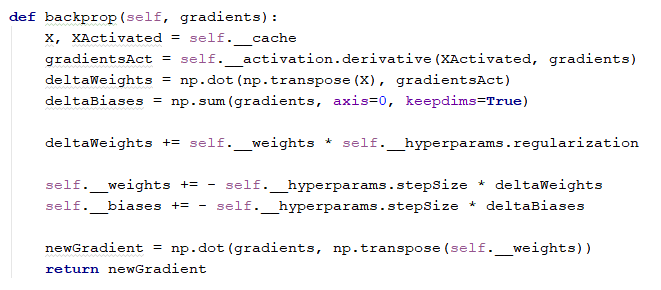
\includegraphics[width=15cm]{hidden_backprop}
	\caption{\label{fig:hidden_backprop} Operatia backprop a stratului Hidden}
	\end{figure}

	Operatia backprop a stratului de tip Convolution:
	\begin{itemize}
	\item	Conceptul propagarii este asemanator celui de tip Hidden. Diferenta va fi facuta la modul in care datele si derivatele sunt reprezentate. Vom reutiliza operatia col2im pentru a readuce datele in starea initiala dupa proceserea acestora.
	La finalul etapi de propagare a stratului de tip Convolution, filtrele vor avea modificarile aduse de catre functia de eroare. (Vezi Fig. \ref{fig:conv_backprop})
	\end{itemize}

	\begin{figure}[H]
	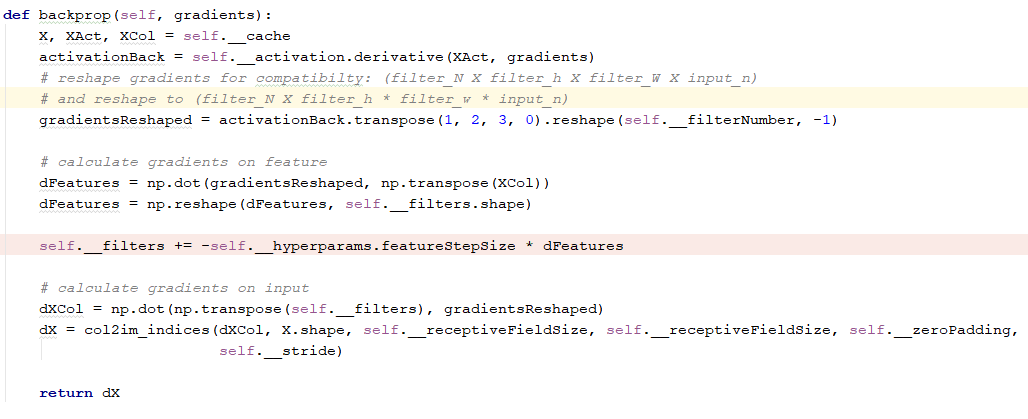
\includegraphics[width=17cm]{conv_back}
	\caption{\label{fig:conv_backprop} Operatia backprop a stratului de Convolution}
	\end{figure}

	Configurarea arhitecturii a fost conceputa sa urmareasca un sablon cat mai simplu. Definirea straturilor si crearea lor va fi realizata prin metoda addLayer al clasei LayersBuilder. Metoda primeste un parametru ce reprezinta tipul de strat ce se doreste a fi creat si un dictionar ce reprezinta parametrii necesari construirii tipului respectiv de strat. Scopul clasei LayersBuilder este de a usura crearea arhitecturii modelului prin izolarea logicii de construire si concatenare a tipurilor de straturi. (vezi Fig. \ref{fig:add_layers})	
	
	\begin{figure}[H]
		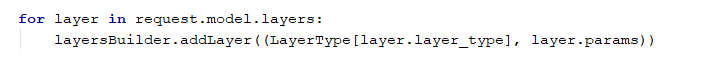
\includegraphics[width=17cm]{add_layers}
		\caption{\label{fig:add_layers} Adaugarea straturilor}
	\end{figure}

	Logica din spate a clasei LayerBuilder se ocupa de ordinea in care straturile sunt adaugate, de  compatibilitatile dintre straturi, de respectarea unor constrangeri si de validare.
	
	Primul pas in construirea straturilor este de a aduna informatii despre structura straturilor, cum ar fi adancimea totala pe care o vom aveam, datorata straturilor de convolutie si a filtrelor,  numarul de reduceri de dimensiune pe care le vom aplica prin straturile de tip Pooling si numarul de straturi de tipuri Hidden. Acestea sunt necesare pentru construirea modelului, dat fiind faptul ca straturile vor avea o dependenta stransa intre ele.  (vezi Fig. \ref{fig:layer_builder})
	
	\begin{figure}[H]
		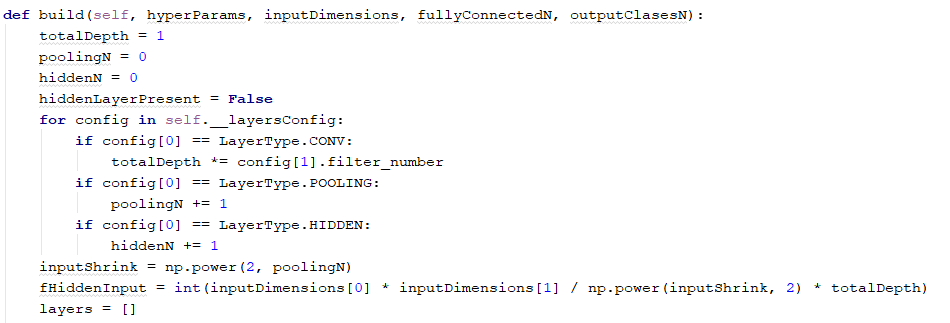
\includegraphics[width=17cm]{layer_builder}
		\caption{\label{fig:layer_builder} Pregatirea datelor; metoda build}
	\end{figure}
	
	\vfill
	

	Dupa ce au fost adunate desule informatii generale legate de structura modelului, vom incepe etapa de constructie a modelului, prin crearea unei liste de obiecte de tip Layer. Parametrii de regularizare si functia de activare vor fi transmise ca si parametri la momentul initializarii tipului de strat. Dupa ce lista a fost construita cu succes,  va fi returnata spre a fi folosita de obiectul de tip Model. (Vezi Fig. \ref{fig:actual_build})
	
	
	\begin{figure}[H]
		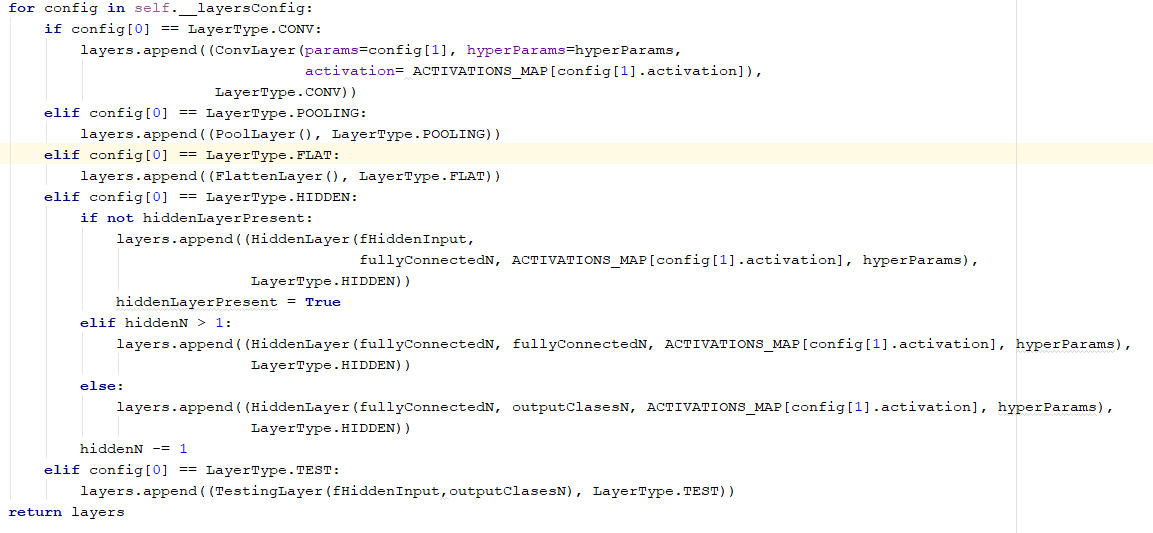
\includegraphics[width=17cm]{actual_build}
		\caption{\label{fig:actual_build} Constructia sirului de straturi}
	\end{figure}

	\newpage

	Dupa ce avem lista de straturi consistent configurata, vom crea un obiect de tip Model, entitatea care va modela parametrii. (vezi Fig \ref{fig:train})
	
	\begin{figure}[H]
		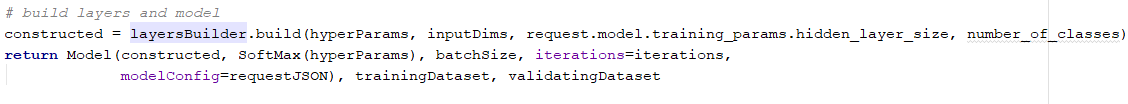
\includegraphics[width=17cm]{train}
		\caption{\label{fig:train} Crearea modelului si antrenarea sa}
	\end{figure}
	

\end{document}